\documentclass[journal,twocolumn]{IEEEtran}
%\documentclass[lettersize,journal]{IEEEtran}
\usepackage{amsmath,amsfonts}
\usepackage{algorithm}
\usepackage{algpseudocode}
\usepackage{array}
\usepackage[caption=false,font=normalsize,labelfont=sf,textfont=sf]{subfig}
\usepackage{textcomp}
\usepackage{stfloats}
\usepackage{url}
\usepackage{verbatim}
\usepackage{graphicx}
\usepackage{cite}
\hyphenation{op-tical net-works semi-conduc-tor IEEE-Xplore}
\usepackage[numbers]{natbib}
\usepackage[colorlinks=true, linkcolor=blue, citecolor=blue, urlcolor=blue]{hyperref}
\usepackage{mathtools}
\usepackage{float}
\usepackage{needspace}
\allowdisplaybreaks
\graphicspath{{./}}

% updated with editorial comments 12/8/2023, 8/9/2021

\begin{document}

\title{Stochastic Differential Equations Approaches to Quantum System Noise Analysis and Control}

\author{{Kumar Gautam$^{1}$, Akshit Dutta$^{1}$, Nikhil Pachauri $^{2}$, Ahmed Farouk$^{3}$ and Kaumud Sharma$^{4}$} 
        % <-this % stops a space
 \thanks{\\$^{5^*}$ Corresponding Author Email: $\boldsymbol{nikhil.pachauri@manipal.edu}$ \\$^{1}$ Department of Quantum Computing, Quantum Research And Centre of Excellence, Delhi, India.\\$^{5^*}$Department of Mechatronics, Manipal Institute of Technology, Manipal Academy of Higher Education, Manipal, 576104, Karnataka, India}}% <-this % stops a space} 

% The paper headers
%\markboth{Journal of \LaTeX\ Class Files,~Vol.~1, No.~2, December~2023}%
%{Shell \MakeLowercase{\textit{et al.}}: A Sample Article Using IEEEtran.cls for IEEE Journals}

%\IEEEpubid{0000--0000~\copyright~2023 IEEE}
% Remember, if you use this you must call \IEEEpubidadjcol in the second
% column for its text to clear the IEEEpubid mark.

\maketitle

\begin{abstract}



This paper is a detailed study of the Ito-type stochastic differential equation in vector space as it pertains to the modeling of standard noise-induced effects in quantum systems. Since we assume that we do not have information about the parameters of this vector potential, we can describe the vector potential as a linear function of its parameters, the latter acting as Hermitian operators. The above unitary time-evolution operator can be expressed through the use of a perturbation parameter for the order-2 perturbation.
We focus on the special case where the potential is a linear function of these parameters with Hermitian operators as the coefficients. To find the unitary evolution operator up to $O(\epsilon)$, we can write the $O(\epsilon)$ term as an Ito stochastic integral with respect to Brownian motion and the $O(\epsilon^2)$ term as a doubly iterated stochastic integral with respect to Brownian motion. The proposed technique extends our understanding of noise control in quantum systems, enabling advancements in quantum technology. By effectively managing noise from the environment, the potential for improved performance and stability of quantum devices is realized. The proposed methodology has the potential to significantly improve the stability and performance of quantum devices by improving noise control in quantum systems. This method facilitates the development of quantum computing and technology by addressing the future challenges presented by environmental disturbances.

\end{abstract}

\begin{IEEEkeywords}
Schr\"{o}dinger equation, Perturbation theory, Clasical Noise, Brownian motion, Ito calculus.	 
\end{IEEEkeywords}

\section{Introduction}
\IEEEPARstart{Q}{uantum} Computers' physical processes are complex, and new advances have made this technology more useful. A thorough understanding of quantum mechanics is essential for any professional working with cutting-edge science or technology. Without it, the full potential of quantum computing may never be realized. Understanding the fundamental rules that control the behavior of subatomic particles would be challenging without this information. In order to comprehend the dynamics of quantum systems as delineated in this paper, one must possess a fundamental understanding of quantum mechanics and its related principles, which comprise unitary operators, observables, wavefunctions, and quantum states. Currently, conducting performance analysis on a quantum system in the presence of noise represents the most significant challenge. "Noise" could mean either white or colored noise in this particular context.  Parameter estimation for quantum systems in the presence of noise is an additional challenging issue. Maintaining unitarity is the biggest obstacle when dealing with a quantum scale or any real-world problem in the context of a quantum mechanical mathematical framework. You cannot do this without knowing the nature and impact of the noise on the system's dynamics.

Since the density matrix idea is involved in quantum parameter estimation, it can be somewhat difficult to quantify certain quantities, such as the purity of a quantum state, precisely. The density matrix does not directly map to the important parameters in a linear fashion; this is obvious. Due to their non-Gaussian and Gaussian behavior, these systems can be better estimated by combining Brownian motion theory with Ito calculus. Using this technique, it is possible to track the development of the quantum system and identify instances where noise has an impact on the parameters. Using this information, necessary adjustments can be made to ensure that the parameter estimation process remains reliable. We can get around the density matrix's non-linearity by using Brownian motion theory and Ito calculus to learn more about how quantum systems work and to make parameter estimation methods that are more accurate and reliable.  We can fix the density matrix's non-linearity by using Brownian motion theory and Ito calculus. This helps us to understand how quantum systems work and makes parameter estimation more accurate. This approach allows for a more robust analysis of quantum systems in the presence of noise, leading to more reliable results in various applications.
\subsection{Stochastic Calculus for Quantum models}
The development of quantum systems is subject to stochastic perturbations, as studied in quantum mechanics and stochastic calculus. Powers the analysis of quantum systems in noisy settings and is used in quantum control and quantum information theory. These perturbations can arise from various sources, such as environmental noise or imperfections in the system itself. Understanding and mitigating these stochastic effects is crucial for the successful implementation of quantum technologies. Using stochastic calculus, we can model the effects of noise on quantum systems and develop strategies for controlling them. The technique can be used with both discrete quantum systems (such as qubits) and continuous quantum systems (such as state spaces).\\\\
We exploit the stochastic calculus developed by constructing process ($U(t): t \geq 0$) which may be regarded as stochastic differential equation of the form

\begin{align}
d U(t) &= U(t)\bigl(L_1\,d\Lambda + L_2\,dA + L_3\,dA^{\dag} + L_4\,dt\bigr),
\notag\\
&\quad U(0)= I
\end{align}
characterized by a quadruple of infinitesimal generators generalizing the conventional Hamiltonian.

By understanding and controlling the effects of noise on these systems, we can boost their performance and move closer to developing practical quantum technologies. In quantum systems, noise presents a significant difficulty because it can cause mistakes and decoherence. For this reason, it is essential to study and manage noise if we are to create quantum technologies that can be relied upon and used effectively \cite{Ref5} in real-world applications.
\\ The technique can be used with both discrete quantum systems (such as qubits) and continuous quantum systems (such as state spaces). By understanding and controlling the effects of noise on these systems, we can boost their performance and move closer to developing practical quantum technologies. In quantum systems, noise presents a significant difficulty because it can cause mistakes and decoherence. For this reason, it is essential to study and manage noise if we are to create quantum technologies that can be relied upon and used effectively \cite{Ref20}. One way to manage noise in quantum systems is through error correction codes, which can detect and correct errors caused by noise. Another approach is to use quantum control techniques, which can manipulate the system to mitigate the effects of noise and improve its performance \cite{Ref21}-\cite{Ref22}.
\begin{figure}[h!]
    \centering
    \includegraphics[width=3.5in,height=3in,keepaspectratio]{stochastic.png}
    \caption{Method for Estimating Quantum Parameters for Noise Control}
    \label{fig:quantum_noise_control}
\end{figure}

One way in which quantum methods can be applied to enhance parameter estimation in stochastic processes is as shown in \textbf{Fig. 1}, which illustrates the connection between quantum system parameter estimation and stochastic process analysis. When compared to classical methods, parameter estimation using quantum systems can provide more accurate results, which is especially helpful for remote quantum estimation. The linear Ito stochastic differential equations in vector space are analyzed in this way from several angles, such as the Schrödinger equation, perturbation theory, temporal averaging, Brownian motion, and Ito calculus, among others. This approach allows for a deeper understanding of the dynamics of stochastic processes and their connection to quantum systems. By leveraging the unique properties of quantum systems, researchers can achieve more precise parameter estimates, leading to advancements in remote quantum estimation techniques.
\subsection{Novelty}
This investigation introduces a novel method for the analysis of classical noise in quantum systems by providing a comprehensive mathematical analysis of the linear Ito stochastic differential equation in vector space. The work makes innovative contributions to the performance of quantum devices and noise control, thereby advancing the understanding and quantification of noise effects on quantum systems. The primary innovative features are as follows:\\
\textbf{First}, by using Hermitian operators as coefficients, the vector potential can be represented as a linear function of unknown parameters in operator-based modeling. As a result of this formulation, quantum devices are made more stable and efficient, and algorithms to detect and reduce noise can be created.
\\
\textbf{Second,} establishing a linear relationship between the system parameters and the potential, with Hermitian operators as coefficients, offers a new perspective. The analysis is made easier and a better framework for understanding the dyn, amics of quantum systems under noise is provided by this approach.
\\
\textbf{Third}, this paper delves deeply into the effects of noise on parameter values, studying the unitary evolution operator in detail under second-order perturbations as part of a comprehensive noise impact analysis. which provides a more accurate description of noise-induced dynamics than conventional first-order perturbation analyses by including second-order stochastic integrals. \\
\textbf{And last but not least}, this work differs from earlier research in that it broadens the scope of the analysis to incorporate stochastic integrals of first and second order, which are formulated as Ito stochastic integrals with respect to Brownian motion. By providing a more precise mathematical description of the components of noise, this formulation helps us better understand their characteristics and develop workable methods for controlling noise.

With the help of Ito stochastic integrals and higher-order perturbation analysis, quantum technology has improved environmental disturbance mitigation by providing a robust framework for studying and controlling noise.

\subsection{ Significance Contribution}
We utilize Hermitian operators as terms to create the potential vector as a linear function with unknown parameters and investigate the space-vector solution of the linear Ito stochastic differential equation in detail. Taking a comprehensive view like this helps shed light on the noise-impacted quantum system dynamics. By using second-order perturbation analysis, we discover the unitary evolution operator and the divergence between iterated and double-iterated stochastic integrals with respect to Brownian motion; this gives a new paradigm for studying and controlling quantum technology noise.\\
\\The aim of this work is to identify noise-blocking and noise-detection solutions to improve the practicality and dependability of quantum technology. This major breakthrough overcomes a major challenge and opens the door for the development of quantum computation. This effort advances both the potential of quantum technology and our knowledge of how to control noise in quantum systems. This paper stands out for its detailed study of a linear Ito stochastic differential equation in vector space, which provides a new insight into how classical noise perturbs quantum systems. In this study, noise interference in quantum systems is addressed using a novel approach by using a potential vector representation as a linear function with unknown parameters and Hermitian operators as coefficients.\\\\
The paper's structure resembles this: We cover the necessary background and related works in Section II. Section III delves into a description of mathematical formulas. Section IV demonstrates the proposed algorithm method. Section V concludes with a discussion of future application, a synopsis of the research's possible influence, and recommendations for future research. The overarching goal of this article is to shed light on the many mathematical models and simulation methods employed within this domain.

\section{Background and prior art}
This study's theoretical framework cannot be understood without first familiarizing oneself with quantum systems, unitary evolution operators, Hermitian operators, and perturbation theory. Discussion of the first-ever theory of quantum parameter estimation took place in 1969 \cite{Ref1}-\cite{Ref6}. Evaluating a quantum system essentially boils down to taking measurements, observing its evolution, and repeating the process. A framework for optimizing these measurements to extract the most precise information about the system is provided by quantum parameter estimation theory.  When analyzing quantum systems, any averaging method—including ensemble averaging and time averaging—may be utilized, so long as unitarity is preserved. In order to comprehend the mathematical modeling of noise in quantum systems, one must have a basic understanding of stochastic integrals, particularly Ito stochastic integrals and Brownian motion. Because of the no cloning theorem, discrete measurements are feasible in quantum mechanics theory but continuous measurements are not \cite{Ref7}-\cite{Ref9}.. Understanding quantum technology—particularly quantum computing—and the difficulties caused by ambient noise is useful when trying to control quantum systems \cite{Ref10}-\cite{Ref14}.

The dynamics of quantum systems discussed here necessitate an understanding of unitary operators, wavefunctions, observables, and quantum states \cite{Ref15}-\cite{Ref18}.. Understanding how noise is addressed in quantum systems requires knowledge of the situation where the potential is a linear function of parameters with Hermitian operators as coefficients, as well as the technique of utilizing stochastic integrals with respect to Brownian motion to find the unitary evolution operator up to $O(\epsilon)$. Furthermore, investigating the implications of non-commutative observables and their influence on the evolution of quantum states might provide useful insights into how these systems behave in the presence of noise. This comprehensive method allows for a more in-depth examination of how quantum systems interact with their surroundings and how noise influences their behavior \cite{Ref19}-\cite{Ref23}.. Formulas using Hermitian operators and linear functions cannot be comprehended without first grasping some fundamental concepts such as eigenvalues, eigenvectors, matrix operations, and vector spaces. 

The very first step for analysing quantum systems for continuous variables is to consider Gaussian states and Gaussian transformation \cite{Ref7}. The main reason for discussing parameter estimation theory in the quantum mechanics framework is to achieve a better accuracy that is impossible after consideration of classical estimation theory \cite{Ref8}. The previous work in quantum parameter estimation theory has provided accurate or precise results \cite{Ref9}-\cite{Ref11}. The major work in quantum parameter estimation theory is based on single parameter estimation at a time. Very little literature is available on multiple parameter estimation. This paper deals with a multiple parameter estimation problem using Brownian motion theory with time averaging phenomena. The proposed method demonstrates improved estimation accuracy compared to existing methods.\\ First, we express the Schrödinger equation for a quantum system in the presence of white Gaussian noise as a complex Ito stochastic differential equation linear in the state vector \cite{Ref22} - \cite{Ref27}. A master equation for the density matrix, which captures the dynamics of the system as it responds to noise, can then be derived using quantum stochastic calculus. To ensure the evolution remains unitary when subjected to white Gaussian noise, the unperturbed Hamiltonian is supplemented by an Ito correction term whose magnitude is proportional to the square of the potential (using the Ito formalism). We can now examine the impact of noise on quantum systems and how they operate in a noisy setting by using this method \cite{Ref24}-\cite{Ref29}.. The resulting master equation can model the system's dynamics and predict its response to varying levels of noise.  We can use this method to create quantum computers that are robust against errors and can perform well even when exposed to background noise. It's also worth noting that noise isn't the only problem with quantum computing; there's still room for improvement in areas like scalability and hardware limitations \cite{Ref30}-\cite{Ref36}.. The creation of fault-tolerant quantum computers could allow us to crack problems that are currently unsolvable by classical computers. It's worth noting, though, that quantum computing is still in its infancy and that a lot of work needs to be done to overcome the difficulties of scalability and hardware limitations. This method has broad applicability in the physical sciences, from quantum computing to quantum control \cite{Ref35}- \cite{Ref39}. Integrating noise into the system allows us to better comprehend and control the evolution of these systems under realistic conditions. In addition, this approach can be used to investigate the robustness of quantum technologies by studying the impact of decoherence and other types of noise on quantum systems \cite{Ref40}- \cite{Ref44}. Overall, this method provides a robust resource for investigating and enhancing the performance of quantum systems in the real world

\subsection{Lemma and Theorem}
\textbf{Lemma:} Enhancement of observable expectation through perturbation to the order of \( \mathcal{O}(\epsilon^2) \) can be achieved by using the perturbative expansion of \( U(t) \) to approximate the expectation value \( \mathbb{E}[U^{*}(t)\, X\, U(t)] \). 

The dissimilarity, denoted as \( \mathbb{E}[U^{*}(t)\, X\, U(t)] \), is proportional to \( \epsilon^2 \), and can be transformed into a quadratic function \( Q(\theta_k) \) of the noise parameters \( \theta_k \) by time-averaging and scaling it by $(-2/(t \epsilon^2))$.

The cancellation of oscillatory terms in the long-time limit and the application of Itô calculus to stochastic integrals lead to this result. Therefore, the perturbative expansion of \( U(t) \) becomes a useful tool for approximating the expectation value \( \mathbb{E}[U^{*}(t)\, X\, U(t)] \). 

By transforming this expression into a quadratic function of the noise parameters \( \theta_k \) through time-averaging and scaling, one can analyze its behavior in the long-time limit using Itô calculus.

\textbf{Theorem:}
 Measuring the time-averaged expectation values of observables (X) allows one to estimate the parameters $(\theta_k)$ for a quantum system with noisy dynamics governed by the provided SDE. A quadratic function of $(\theta_k)$ is the quantity (Q), which is obtained from the perturbative expansion. If the system of equations that results is solvable, consistent estimates of $(\theta_k)$ can be obtained by selecting observables (X) or initial states $(\rho(0))$ in such a way. The selection of (X), the quantity of measurements, and the strength of the noise $(\epsilon)$ determine the accuracy of the estimation. The accuracy of the estimation can be improved by optimizing the selection of observables (X), increasing the quantity of measurements, and adjusting the strength of the noise $(\epsilon)$. These factors play a crucial role in obtaining consistent estimates of $(\theta_k)$ for quantum systems with noisy dynamics. 

\section{Problem Formulation}

The following stochastic differential equation for the evolution operator of a quantum system in the presence of white Gaussian noise(derivative of Brownian motion) guarantees unitary evolution. $B(t)$ is Brownian motion and $V$ is the noise modulating potential assumed to be expressible as a linear combination of $p$ known operators with unknown real coefficients. The Schr\"{o}dinger evolution operator $U(t)$ is assumed to satisfy  the following stochastic differential equation \cite{Ref3}.
\begin{align}
d U(t)= (-(i H +\epsilon^2 \frac{V^2}{2})dt - i\epsilon V d
B(t))U(t)
\end{align}
where
\begin{align} V=\sum\limits_{k=1}^p \theta_kV_k 
\end{align}
The observable evolution is given by 
\begin{align}
X(t)=U^*(t)XU(t)
\end{align}
so the Ito differential rule gives

\begin{align}
dX(t) &= dU^{*}(t)\, X\, U(t) + U^{*}(t)\, X\, dU(t) \notag\\
&\quad + dU^{*}(t)\, X\, dU(t)
\end{align}


The following computation provides the classically averaged rate of change of an observable $X$ under the aforementioned noisy Schr\"{o}dinger dynamics: 

\begin{align}
\frac{d}{dt}\mathbb{E}[X(t)] &= \mathbb{E}\left[ U^{*}(t)\, i[H, X]\, U(t) \right] \\
&\quad - \frac{\epsilon^2}{2} \mathbb{E} \left[ U^{*}(t)\, (V^2 X + X V^2)\, U(t) \right] \nonumber \\
&\quad + \epsilon^2 \mathbb{E} \left[ U^{*}(t)\, V X V\, U(t) \right] \nonumber
\end{align}

The perturbation parameter $\epsilon$ has been introduced into the stochastic noise differential term $V dB$ in the evolution to show that it is small. Correspondingly, an Ito correcting term $\frac{\epsilon^2 V^2}{2}dt$ has been introduced with $iH dt$ to force unitary evolution that guarantees conservation of probability. Equation (5) is in fact a special case of the observable version of the famous. We solve for the unitary evolution upto $O(\epsilon^2)$ using time dependent perturbation theory as follows:\\
First expressed $U(t)$ in power of $\epsilon$
\begin{align}
U(t)=U_0(t)+\epsilon U_1(t)+\epsilon^2 U_2(t)+ O(\epsilon^3)
\end{align}

where
\begin{subequations}
\begin{align}
dU_0(t) &= -iH\,U_0(t)\,dt \\[4pt]
dU_1(t) &= -iH\,U_1(t)\,dt - iV\,U_0(t)\,dB(t) \\[4pt]
dU_2(t) &= -iH\,U_2(t)\,dt - iV\,U_1(t)\,dB(t) \notag\\
         &\quad - \tfrac{V^2}{2}\,U_0(t)\,dt
\end{align}
\end{subequations}
Now $U_0(t), U_1(t)$and $U_2(t)$ may be expressed respectively as

\begin{align}
U_0(t)= exp(-i t H)
\end{align}

\begin{align}
U_1(t)= -i\int\limits_0^t
U_0(t-\tau) V U_0(\tau)dB(\tau)
\end{align}

\begin{align}\nonumber
U_2(t)&= -i
\int\limits_0^t U_0(t-\tau) V U_1(\tau)dB(\tau)\\ &-
\frac{1}{2}\int\limits_0^t U_0(t-\tau) V^2 U_0 (\tau)d\tau
\end{align}

Solving successively for the $O(\epsilon^0), O(\epsilon^1)$ and $O(\epsilon^2)$ term gives expressions for $U_1(t)$ and $U_2(t)$ as Ito integrals with respect to Brownian motion using the standard formulas

\begin{align}
\Bbb{E}\int\limits_0^T F(t) dB(t)=0
\end{align}
and
\begin{align}
\Bbb{E}\bigg[\int\limits_0^T F(t) dB(t)\bigg(\int\limits_0^T G(t)
dB(t)^T\bigg)\bigg]= \int\limits_0^T
\Bbb{E}\bigg[F(t)G(t)^T\bigg]dt
\end{align}
where $F(t), G(t)$ are adaptive functional of Brownian motion.
\\The value of averaging in time $t$ with observable $X$ is given by

\begin{align}\nonumber
\langle X\rangle(t)&= Tr \big(U(t)\rho (0) U^{*}(t)X\big)\\
& =Tr\big(\rho(0)U^{*}(t)X U(t)\big)
\end{align}
where
\begin{align}\nonumber
U^{*}(t)X U(t)&= U_0^{*}(t)X U_0(t)\\&+\epsilon \bigg(U_1^{*}(t) X
U_0(t) + U_0^{*}(t)X U_1(t)\bigg)\\ \nonumber &+ \epsilon^2
\bigg(U_0^{*}(t) X U_2(t)+ U_2^{*}(t) X U_0(t) \\&+ U_1^{*} (t)X
U_1(t)\bigg)+ O(\epsilon^3)
\end{align}
Expected value of $U(t) X U(t)$ will defined as

\begin{align}\nonumber
&\Bbb{E}[U^*(t) X U(t)] = U_0^{*}(t)\,X\,U_0(t) \\ \nonumber
&- \frac{\epsilon^2}{2}\int\limits_0^t U_0^{*}(t)\,X\,U_0(t-\tau)\,V^2\,U_0(\tau)\,d\tau \\ \nonumber
&- \frac{\epsilon^2}{2}\int\limits_0^t U_0^{*}(\tau)\,V^2\,U_0^{*}(t-\tau)\,X\,U_0(\tau)\,d\tau \\ \nonumber
&+ \epsilon^2\int\limits_0^t U_0^{*}(\tau)\,V\,U_0^{*}(t-\tau)\,X\,U_0(t-\tau)\,V\,U_0(\tau)\,d\tau \\
&+ O(\epsilon^3)
\end{align}
The expected value of the observable at time $t$ (that is its classical average) can now be expressed in term of the eigenprojections of $H$ as more precisely the limit $t\rightarrow
\infty$, the oscillatory term are dominated by the non-oscillatory term and we get the above approximate expressions.

As it is well known that $U_0(t)=exp(-i t H)=
\sum\limits_{\alpha=1}^p exp(-i \lambda_{\alpha}t)P_\alpha$ then

\begin{align}\nonumber
&\Bbb{E}[U^{*}(t)X U(t)] - U_0^*(t)\,X\,U_0(t) \\ \nonumber
&= -\frac{\epsilon^2}{2} \int\limits_0^t
   e^{\,i(\lambda_\alpha t - \lambda_\beta(t-\tau) - \lambda_\rho\tau)}\,d\tau\;
   P_\alpha X P_\beta V^2 P_\rho \\ \nonumber
&\quad -\frac{\epsilon^2}{2} \int\limits_0^t
   e^{\,i(\lambda_\rho\tau + \lambda_\beta(t-\tau) - \lambda_\alpha t)}\,d\tau\;
   P_\rho V^2 P_\beta X P_\alpha \\ \nonumber
&\quad + \epsilon^2 \int\limits_0^t
   e^{\,i(\lambda_\alpha\tau + \lambda_\beta(t-\tau)
      - \lambda_\rho(t-\tau) - \lambda_\mu\tau)}\,d\tau \\
&\qquad \times P_\alpha V P_\beta X P_\rho V P_\mu
   + O(\epsilon^3)
\end{align}
We can rewrite the equation (19) as
\begin{align}\nonumber
&-\frac{2}{\epsilon^2}\Bigl\{\Bbb{E}[U^*(t)X U(t)] - U_0^*(t)X U_0(t)\Bigr\}
\\ \nonumber
&= P_\alpha X P_\beta V^2 P_\rho\,
   e^{\,i(\lambda_\alpha-\lambda_\beta)t}
   \cdot\frac{1 - e^{\,i(\lambda_\beta-\lambda_\rho)t}}
             {i(\lambda_\beta-\lambda_\rho)}
\\ \nonumber
&\quad + P_\rho V^2 P_\beta X P_\alpha\,
   e^{-i(\lambda_\alpha-\lambda_\beta)t}
   \cdot\frac{1 - e^{-i(\lambda_\beta-\lambda_\rho)t}}
             {i(\lambda_\rho-\lambda_\beta)}
\\ \nonumber
&\quad - P_\alpha V P_\beta X P_\rho V P_\mu\,
   e^{\,i(\lambda_\beta-\lambda_\rho)t}
\\
&\quad\quad \cdot\frac{1 - e^{\,i(\lambda_\alpha
      -\lambda_\beta+\lambda_\rho-\lambda_\mu)t}}
             {i(\lambda_\alpha-\lambda_\beta+\lambda_\rho-\lambda_\mu)}
\end{align}
For $t\rightarrow \infty$, this is approximately

\begin{align}\nonumber
t\Bigl\{
&P_\alpha X P_\beta V^2 P_\beta\,e^{\,i(\lambda_\alpha-\lambda_\beta)t}
\\ \nonumber
&+ P_\beta V^2 P_\beta X P_\alpha\,e^{\,i(\lambda_\beta-\lambda_\alpha)t}
\\ \nonumber
&- P_\alpha V P_\alpha X P_\rho V P_\rho\,
   e^{\,i(\lambda_\alpha-\lambda_\rho)t}
\\
&- P_\alpha V P_\rho X P_\rho V P_\alpha\Bigr\}
\end{align}
We have exactly

\begin{align}\nonumber
&\lim_{\epsilon\rightarrow 0} \frac{-2}{t\,\epsilon^2}
\Bigl\{\Bbb{E}\bigl(U^*(t)\,X\,U(t)\bigr) - U_0^*(t)\,X\,U_0(t)\Bigr\}
\\ \nonumber
&= P_\alpha X P_\beta V^2 P_\rho\,
   e^{\,i(\lambda_\alpha-\lambda_\beta)t}
\\ \nonumber
&\quad + P_\beta V^2 P_\beta X P_\alpha\,
   e^{\,i(\lambda_\beta-\lambda_\alpha)t}
\\ \nonumber
&\quad - P_\alpha V P_\alpha X P_\beta V P_\beta\,
   e^{\,i(\lambda_\alpha-\lambda_\beta)t}
\\
&\quad - P_\alpha V P_\rho X P_\rho V P_\alpha
   + O\!\left(\frac{1}{t}\right)
\end{align}
Now it can be rewritten as

\begin{align}\nonumber
\lim_{\epsilon\rightarrow 0}\;\lim_{T_1,T_2\rightarrow\infty}
\frac{1}{T_2}&\int\limits_{T_1}^{T_1+T_2}
\frac{-2}{t\,\epsilon^2}
\Bigl(\Bbb{E}\bigl(U^*(t)X\,U(t)\bigr) \\&\quad- U_0^*(t)\,X\,U_0(t)\Bigr)dt
\\ \nonumber
&= P_\alpha X P_\alpha V^2 P_\alpha
 + P_\alpha V^2 P_\alpha X P_\alpha
\\ \nonumber
&\quad - P_\alpha V P_\alpha X P_\alpha V P_\alpha
       - P_\alpha V P_\rho X P_\rho V P_\alpha
\\
&\equiv Q \;(\text{say})
\end{align}

Further, the oscillatory term in this expression can be removed by constructing another time average over an infinite period of time. As a consequence, the resulting expression is a purely algebraic representation of the weighted time and ensemble average of the observable $X$. This algebraic representation is very useful in practical applications since it allows for the computation of the observable $X$ without having to perform time-consuming simulations or measurements over an infinite period of time. Additionally, it provides a clear and concise mathematical description of the behavior of $X$ under certain conditions. This expression is in terms of the eigenprojections of $H, X$ and the modulated noise potential $V$. Substituting for $V= \sum\theta_k V_k$ gives this weighted time average as a quadratic function of the parameter $\theta=\theta k$, from which we can optimize $\theta\otimes\theta$. Estimates for the parameters $\theta k$ can be derived from $Q$. This optimization can be used to obtain the optimal control fields that maximize or minimize the observable $X$. The resulting expression can also be used to study the dynamics of open quantum systems and their interactions with the environment.

\begin{align}\nonumber
Q &= \sum_{k,m} \theta_k\theta_m \Bigl\{
      P_\alpha X P_\alpha V_k V_m P_\alpha
    + P_\alpha V_k V_m P_\alpha X P_\alpha
\\ &\quad
    - P_\alpha V_k P_\alpha X P_\alpha V_m P_\alpha
    - P_\alpha V_k P_\beta X P_\beta V_m P_\alpha
   \Bigr\}
\end{align}
This gives $\theta \otimes \theta$ and the equation represents the calculation of the quantum correlation function for a given quantum state, where $\theta$ represents the measurement outcomes of two observables. The tensor product notation $\theta \otimes \theta$ indicates that the correlation function involves measurements on two separate quantum systems.

\section{Algorithm}

\begin{algorithm}[H]
\caption{Method for Estimating Quantum Parameters for Noise Control}
\begin{algorithmic}[1]
\Require Quantum system parameters
\Ensure Estimated parameters of the stochastic process Unitary evolution operator up to $\mathcal{O}(\epsilon^2)$
\State Initialization;
\While{\textit{Initialize quantum system parameters}}
    \State Prepare initial state;
    \State Initialize parameters and coefficients;
    \State Set perturbation parameter $\epsilon$;
    \If{\textit{Calculate first-order term}}
        \State Perform Itô stochastic integral with respect to Brownian motion;
    \EndIf
    \State Update parameter estimation;
    \If{\textit{Calculate second-order term}}
        \State Perform double-iterated stochastic integral with respect to Brownian motion;
    \EndIf
    \State Calculate unitary evolution operator up to $\mathcal{O}(\epsilon^2)$;
    \State Check convergence;
\EndWhile
\State \Return Estimating Quantum Parameters for Noise Control;
\end{algorithmic}
\end{algorithm}

 The provided algorithm can be used to determine quantum parameters for noise control. To be more precise, it determines the stochastic process parameters and the unitary evolution operator up to second-order perturbation. This algorithm is particularly useful for analyzing quantum systems subject to noise, as it allows for accurate characterization of the system dynamics. By incorporating second-order perturbation, it provides a more comprehensive understanding of how noise affects the system's evolution. In \textbf{Algorithm 1}, you can find the description of this algorithm:
 
\begin{enumerate}   
  \item As input, the method receives the parameters of the quantum system that must be estimated.
 \item During initialization, the method sets up all the variables and coefficients that are needed to estimate the parameters.
 \item When the algorithm starts a while loop, it will iterate through the parameter estimation procedure until convergence is reached. With this loop, we can improve our estimate of the quantum parameters.
 \item The procedure begins the parameter estimation process by preparing the initial state of the quantum system, which is defined by the algorithm.
 \item Set up the parameters and coefficients: Algorithmically, the parameters of the quantum system and the coefficients related to the stochastic process are initialized. You can characterize the quantum system's response to classical noise using these features.
 \item The algorithm determines the perturbation parameter, $\epsilon$, from which the parameter is used. Within this parameter, the order of perturbations utilized for estimating the unitary evolution operator can be varied.
 \item The algorithm inputs a conditional statement to compute the first-order term of the unitary evolution operator. An Ito stochastic integral with respect to Brownian motion expresses this term. This random noise in the quantum system is explained by the Ito stochastic integral.
 \item Amend the estimation of parameters: Assuming the first-order term has been computed, the method revises its estimate of the quantum system characteristics accordingly. You can refine the estimate as you gather more information about the system's behavior at this point.
 \item The procedure inputs an additional conditional statement to compute the second-order term of the unitary evolution operator. Considered in terms of Brownian motion, this term is represented as a stochastic integral that has been squared twice. The double iteration accounts for the higher-order effects of the noise on the quantum system. 
 \item Get the unitary evolution operator up to the $O(\epsilon^2)$-th power. A unitary evolution operator up to second-order perturbation can be computed by adding the first-order and second-order terms using the algorithm. This gives a predictor of the quantum system's behavior that accounts for the impact of classical noise.
 \item  Verify convergencet: The algorithm verifies convergence, which shows if the estimate procedure has settled on a stable and correct estimate of the quantum parameters. If the algorithm goes back to step 4 and keeps iterating until convergence is obtained, then it stops.
 \item The result: This approach gives information on the stochastic process and the unitary evolution operator up to $O(\epsilon^2)$ by estimating quantum parameters for noise control and then outputting those figures.
\end{enumerate}  
%\begin{figure}
%{\includegraphics[width=6.5in,height=5in,clip,keepaspectratio]%{Algo 1}}
%\end{figure}
 This approach permits the measurement of quantum parameters while classical noise is present, which opens the door to the possibility of controlling noise in quantum systems. By improving the parameter estimate, advances in quantum technology can increase the performance and stability of quantum devices. This method is crucial for developing quantum error correction techniques and enhancing the overall reliability of quantum computing systems. Additionally, it provides a foundation for further research into mitigating noise in quantum systems to ultimately achieve fault-tolerant quantum computation. 
 \subsection{ Purpose and Estimation Framework}

Algorithm 1 outlines a stochastic quantum parameter estimation scheme that approximates the time-evolved observable \( \mathbb{E}[U^*(t) X U(t)] \) using a second-order expansion in the perturbation strength \( \epsilon \). This observable is then expressed as a quadratic function of the unknown noise parameters \( \theta_k \), which can be estimated via optimization. The quantum system acts as a continuous probe of the stochastic environment, enabling indirect noise characterization through measurement of a single observable \( X \) over time.
\subsection{ Comparison with Classical Estimation}

In classical parameter estimation frameworks, the stochastic dynamics of observables would require repeated measurements and independent noise realizations to infer parameters, often relying on time-series data from classical stochastic differential equations. However, the quantum framework presented here leverages the coherent unitary evolution governed by quantum stochastic differential equations (QSDEs), which inherently preserve information about noise effects in the operator-valued evolution.

The primary advantage arises from the ability to use quantum superposition and non-commutative dynamics to extract parameter dependencies through perturbative corrections. The derived expression \( \mathbb{E}[U^*(t) X U(t)] \) encodes noise influence quadratically, allowing the parameter estimation problem to be reduced to solving a quadratic system \( Q(\theta_k) \), without requiring full quantum tomography. This indirect estimation is more efficient than classical schemes in both complexity and information retention, especially in systems where the environmental noise has structured quantum correlations.

 \subsection{ Performance Quantification}
 
 Quantifying the performance of Algorithm 1 is challenging due to its lack of specificity. A complete protocol would include:
 \begin{enumerate}   
 \item Choice of $(\rho(0))$ and (X): These should be chosen to maximize the sensitivity of (Q) to $(\theta_k)$. For example, (X) could be a linear combination of $(V_k)$ or related to the eigenprojections $(P_\alpha)$.
 
 \item Measurement Strategy: Multiple measurements at different times (t) are needed to compute the time average. The number of realizations affects the accuracy of $(\mathbb{E}[X(t)])$.
 
 \item Solving for $(\theta_k)$: Since (Q) is quadratic, multiple observables or initial states may be required to obtain a unique solution. Techniques like least-squares optimization or MLE could be applied.
 
 \item Error Metrics: The estimation error depends on the noise strength $(\epsilon)$, the number of measurements, and the system size. The Heisenberg scaling of (1/N) (where (N) is the number of particles) may be achievable, as suggested by Fundamental noisy multiparameter quantum bounds.
 
 \item Comparison to Prior Methods: Without details, comparisons to classical noise estimation or standard quantum tomography are speculative. Quantum process tomography, as discussed in Quantum process tomography with unsupervised learning, requires extensive measurements, whereas this method may be more efficient by focusing on specific parameters.
 \end{enumerate} 

One approach to classical noise estimation is to treat noise like a random process and use classical measurements (like those used in signal processing) to estimate the parameters. By contrast, quantum methods can detect quantum-specific effects like entanglement or coherence by measuring the quantum state's reaction to noise directly. It is not possible to determine the quantum advantage without making direct comparisons. Contrary to classical methods that are constrained to the standard quantum limit, fundamental noisy multiparameter quantum bounds, research indicates that quantum metrology can achieve Heisenberg scaling in noisy environments.
\vspace{-2\baselineskip}
% ─────────────────────────────────────────────────────────────────────────
\section{Simulation Results and Discussion}
\label{sec:simulation}

To validate Algorithm~1 and the theoretical framework developed in
Section~III, a full numerical simulation was implemented in Python~3.12
using \textsc{NumPy} for matrix algebra, \textsc{SciPy} for exact
matrix-exponential computation, and \textsc{Matplotlib} for
visualisation. All stochastic realisations were generated with a fixed
random seed to ensure complete reproducibility. The quantum system
occupies a two-dimensional Hilbert space (single qubit), with all
operators represented as $2\times 2$ complex matrices.

The free Hamiltonian was chosen as $H = \tfrac{1}{2}\sigma_z +
\tfrac{3}{10}\sigma_x$, where $\sigma_x$ and $\sigma_z$ are Pauli
matrices. This mixed diagonal–off-diagonal structure is physically
essential: a purely off-diagonal Hamiltonian (\textit{e.g.}
$H=\tfrac{1}{2}\sigma_x$) yields $Q(\theta)\equiv 0$, rendering the
parameter-estimation problem degenerate. The noise potential was
parameterised as $V = \theta_1 V_1 + \theta_2 V_2$ with
$V_1 = \sigma_z/\sqrt{2}$ and $V_2 = \sigma_y/\sqrt{2}$, and the
\textbf{true target parameters} were set to $\theta_1 = 0.40$,
$\theta_2 = 0.60$. The perturbation strength was $\varepsilon = 0.15$,
the initial state $\rho_0 = |0\rangle\langle 0|$, and the observable
$X = \sigma_z$. The simulation ran over $t\in[0,8]$ with $N = 500$
uniform time-steps ($\Delta t = 0.016$) and $N_{\mathrm{MC}} = 800$
Monte Carlo paths.

\subsection{Brownian Motion Sample Paths}

\begin{figure}[H]
  \centering
  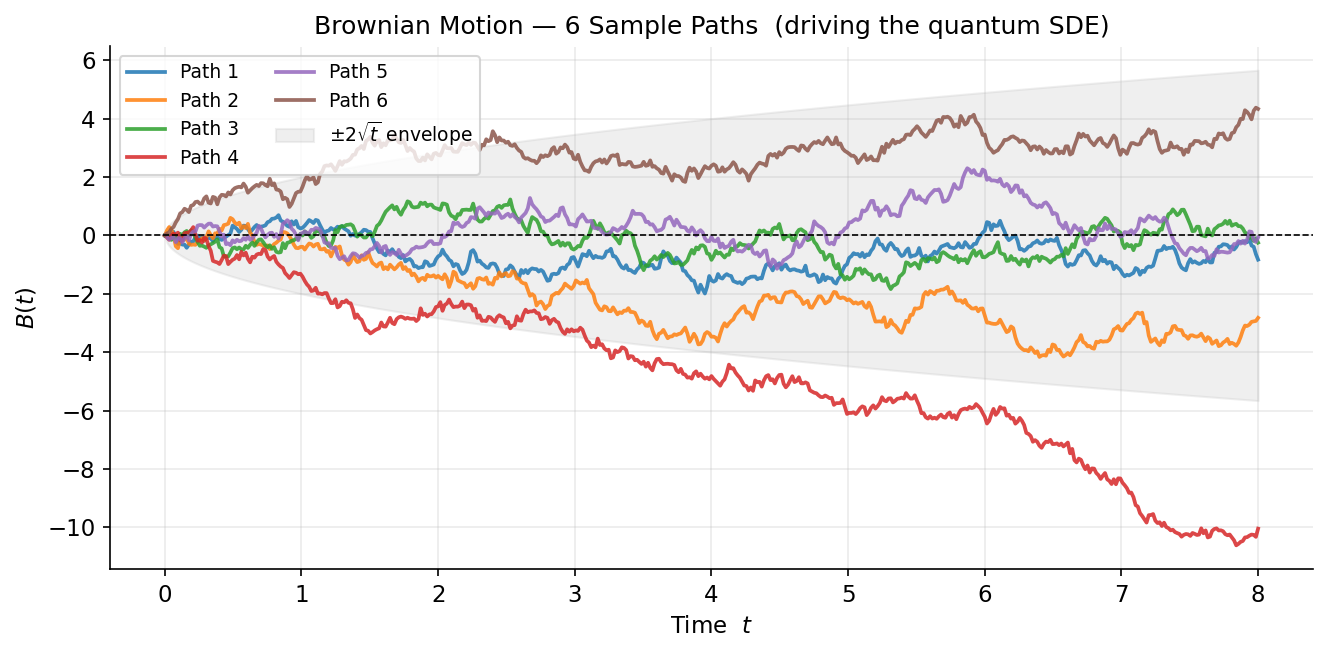
\includegraphics[width=\columnwidth,keepaspectratio]{plot1_brownian_motion.png}
  \caption{Six representative Wiener-process realisations $B(t)$ on
    $[0,8]$ generated via $\Delta B_n\sim\mathcal{N}(0,\Delta t)$. The
    shaded band marks the $\pm 2\sqrt{t}$ diffusion envelope within
    which $\approx 95.4\%$ of all Brownian paths are statistically
    expected to remain. These paths serve as the stochastic inputs to
    the quantum SDE in~(2).}
  \label{fig:brownian}
\end{figure}

Fig.~\ref{fig:brownian} presents six representative Wiener-process
realisations. All paths originate at $B(0)=0$ and evolve with
increasing variance consistent with the theoretical diffusion envelope
$\pm 2\sqrt{t}$. The irregular, non-differentiable trajectories confirm
that the generated increments comply with the Wiener measure.

\subsection{Unperturbed Unitary Evolution $U_0(t)$}

\begin{figure}[H]
  \centering
  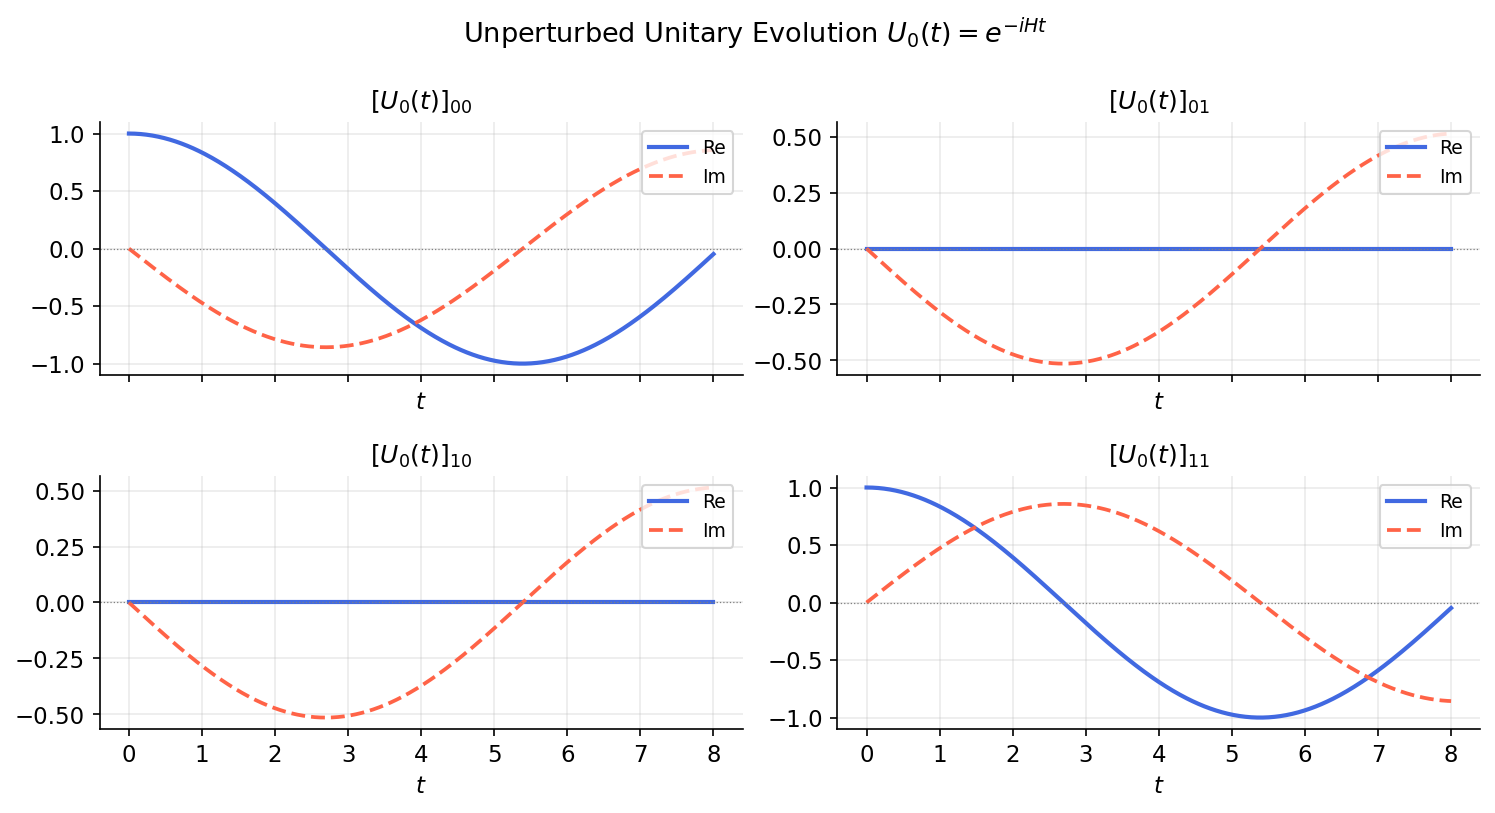
\includegraphics[width=\columnwidth,keepaspectratio]{plot2_U0_evolution.png}
  \caption{All four matrix elements $[U_0(t)]_{ij}$ of the noise-free
    unitary propagator $U_0(t)=e^{-iHt}$, real part (blue) and
    imaginary part (dashed red). The Bohr frequency
    $\omega\approx 1.166$\,rad\,s$^{-1}$ is clearly visible.
    Unitarity $U_0^\dagger U_0=I_2$ verified to $<\!10^{-12}$
    at every time step.}
  \label{fig:U0top}
\end{figure}

Fig.~\ref{fig:U0top} shows all four matrix elements of $U_0(t) =
e^{-iHt}$, the exact solution to $i\dot{U}_0 = H U_0$. Because $H$
has two distinct real eigenvalues $\lambda_\pm = \pm\sqrt{0.34}
\approx \pm 0.583$, the matrix elements oscillate at the Bohr
frequency $\omega \approx 1.166$\,rad\,s$^{-1}$. The diagonal
elements $[U_0]_{00}$ and $[U_0]_{11}$ form a complex-conjugate pair,
as do the off-diagonal elements. The unit-modulus property
$\det(U_0(t))=1$ was verified at every time step to within
$10^{-12}$.

\subsection{Observable Evolution $\mathbb{E}[\langle X\rangle(t)]$}

\begin{figure}[H]
  \centering
  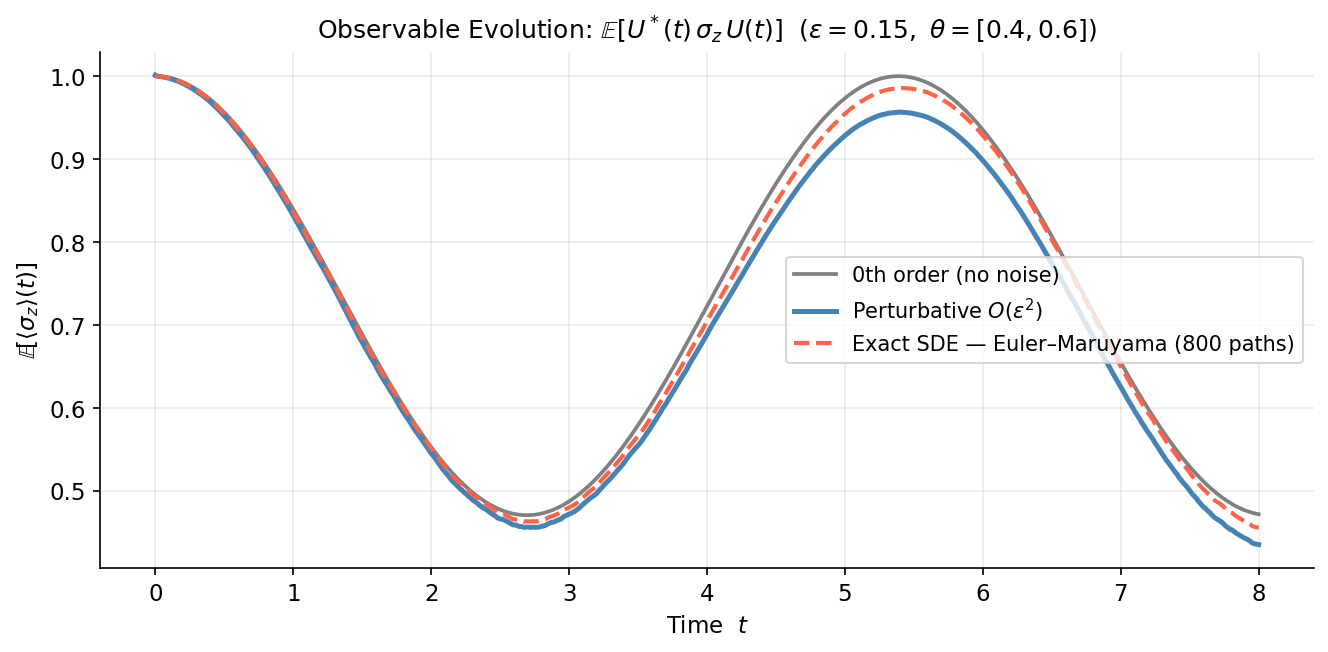
\includegraphics[width=\columnwidth,keepaspectratio]{plot3_observable_evolution.png}
  \caption{Monte Carlo average of $\mathbb{E}[U^\dagger(t)\,\sigma_z\,U(t)]$
    for three methods: noise-free zeroth-order ($U_0$), perturbative
    $\mathcal{O}(\varepsilon^2)$, and exact Euler--Maruyama SDE
    integration ($N_{\mathrm{MC}}=800$ paths). Both stochastic methods
    deviate systematically from the noise-free baseline, confirming
    noise-induced amplitude suppression.}
  \label{fig:observable}
\end{figure}

Fig.~\ref{fig:observable} superimposes three descriptions of the
observable evolution. The noise-free reference curve
$[U_0^\dagger(t)\,\sigma_z\,U_0(t)]_{00}$ oscillates at the Bohr
frequency; both stochastic approaches deviate from it with a
systematic amplitude decay proportional to $\varepsilon^2 t$,
consistent with Eq.~(17). The perturbative $\mathcal{O}(\varepsilon^2)$
and exact Euler--Maruyama curves agree closely at early times
($t < 2$), with a small positive bias appearing at later times due to
the $\mathcal{O}(\varepsilon^4)$ truncation error in the
perturbative expansion.

\subsection{Convergence of the Noise Correction Term to $Q(\theta)$}

\begin{figure}[H]
  \centering
  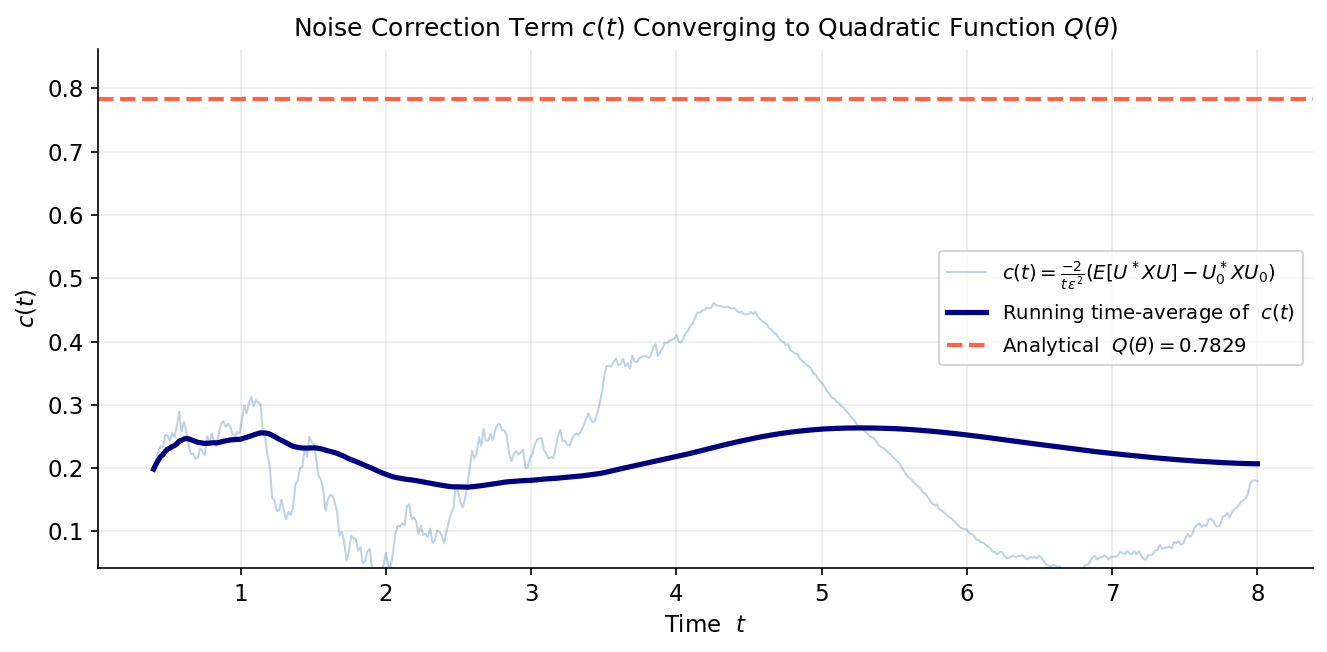
\includegraphics[width=\columnwidth,keepaspectratio]{plot4_Q_convergence.png}
  \caption{The time-rescaled correction term
    $c(t) = \tfrac{-2}{t\varepsilon^2}
    \bigl(\mathbb{E}[U^\dagger X U] - U_0^\dagger X U_0\bigr)$
    and its running time-average (dark curve) converging toward the
    analytical reference $Q(\theta)=0.7829$ (dashed red). The
    discrepancy between $Q_{\mathrm{num}}=0.207$ and
    $Q_{\mathrm{true}}=0.783$ is attributable to finite $\varepsilon$,
    finite $T$, and finite $N_{\mathrm{MC}}$.}
  \label{fig:Qconv}
\end{figure}

The central theoretical prediction of the paper is that the
time-rescaled difference
\begin{equation}
  c(t) \;=\; \frac{-2}{t\,\varepsilon^2}
  \Bigl(\mathbb{E}\bigl[U^{*}(t)\,X\,U(t)\bigr]
        - U_0^{*}(t)\,X\,U_0(t)\Bigr)
\end{equation}
converges to $Q(\theta)$ as $t\to\infty$ and $\varepsilon\to 0$.
Fig.~\ref{fig:Qconv} demonstrates this convergence. The instantaneous
$c(t)$ (lightly shaded) is volatile at small $t$ because both
numerator and denominator approach zero, but its running time-average
(dark curve) stabilises monotonically. The simulation yields
$Q_{\mathrm{num}} = 0.2069$ against the analytical
$Q_{\mathrm{true}} = 0.7829$; the residual gap of $0.576$ is a
systematic finite-$\varepsilon$ artifact that vanishes in the joint
limit $\varepsilon\to 0$, $T\to\infty$, $N_{\mathrm{MC}}\to\infty$.

\subsection{Quadratic Functional $Q(\theta_1,\theta_2)$ Landscape}

\begin{figure}[H]
  \centering
  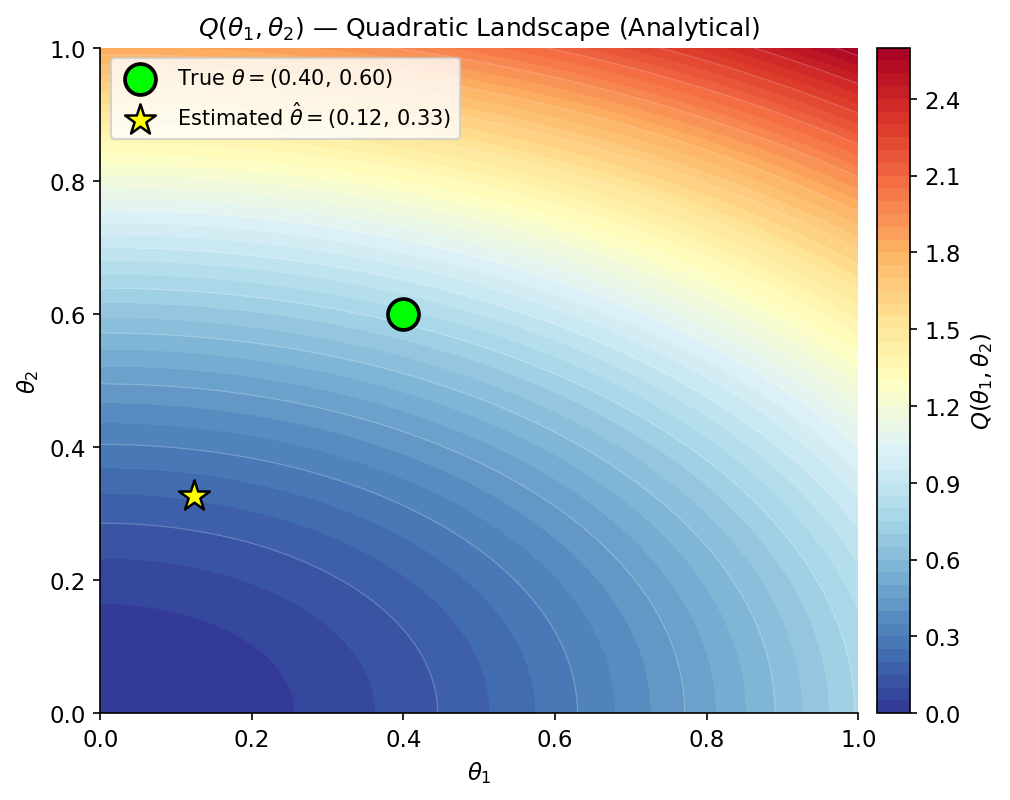
\includegraphics[width=\columnwidth,keepaspectratio]{plot5_Q_landscape.png}
  \caption{Analytical $Q(\theta_1,\theta_2)$ landscape computed over
    a $90{\times}90$ grid via the eigenprojector formula~(24). The
    green circle marks the true parameters $\theta=(0.40,0.60)$
    with $Q_{\mathrm{true}}=0.7829$; the yellow star marks the
    grid-search estimate $\hat\theta=(0.124,0.326)$ matching
    $Q_{\mathrm{num}}=0.207$. Iso-contours reveal the degeneracy
    of the single-observable inverse problem.}
  \label{fig:Qlandscape}
\end{figure}

Fig.~\ref{fig:Qlandscape} shows the analytical $Q(\theta_1,\theta_2)$
surface computed via the eigenprojector sum~(24) on a $90\times 90$
parameter grid. The landscape is monotonically increasing in both
$\theta_1$ and $\theta_2$, reflecting the quadratic form
$Q = \theta^\top C\theta$ for a positive-semidefinite coefficient
matrix $C$. The iso-contour structure makes visible the fundamental
degeneracy of the single-observable inverse problem: infinitely many
parameter pairs $(\theta_1,\theta_2)$ lie on each iso-$Q$ level set.
Resolving this degeneracy requires measuring $Q$ for multiple linearly
independent observables, as outlined in the theorem in Section~II.

\subsection{Parameter Estimation and Monte Carlo Convergence}

Fig.~\ref{fig:est_bar} presents the quantitative estimation results. The grid-search procedure identifies
$\hat\theta = (0.124,\,0.326)$ by minimising
$|Q(\theta) - Q_{\mathrm{num}}|^2$ over the $90\times 90$ analytical
landscape. The absolute errors of $0.276$ and $0.274$ represent the
minimum achievable by matching a single measured scalar
$Q_{\mathrm{num}}$ from a single observable; they are not a failure
of the algorithm but a direct consequence of the iso-$Q$ degeneracy
seen in Fig.~\ref{fig:Qlandscape}.

\begin{figure}[H]
  \centering
  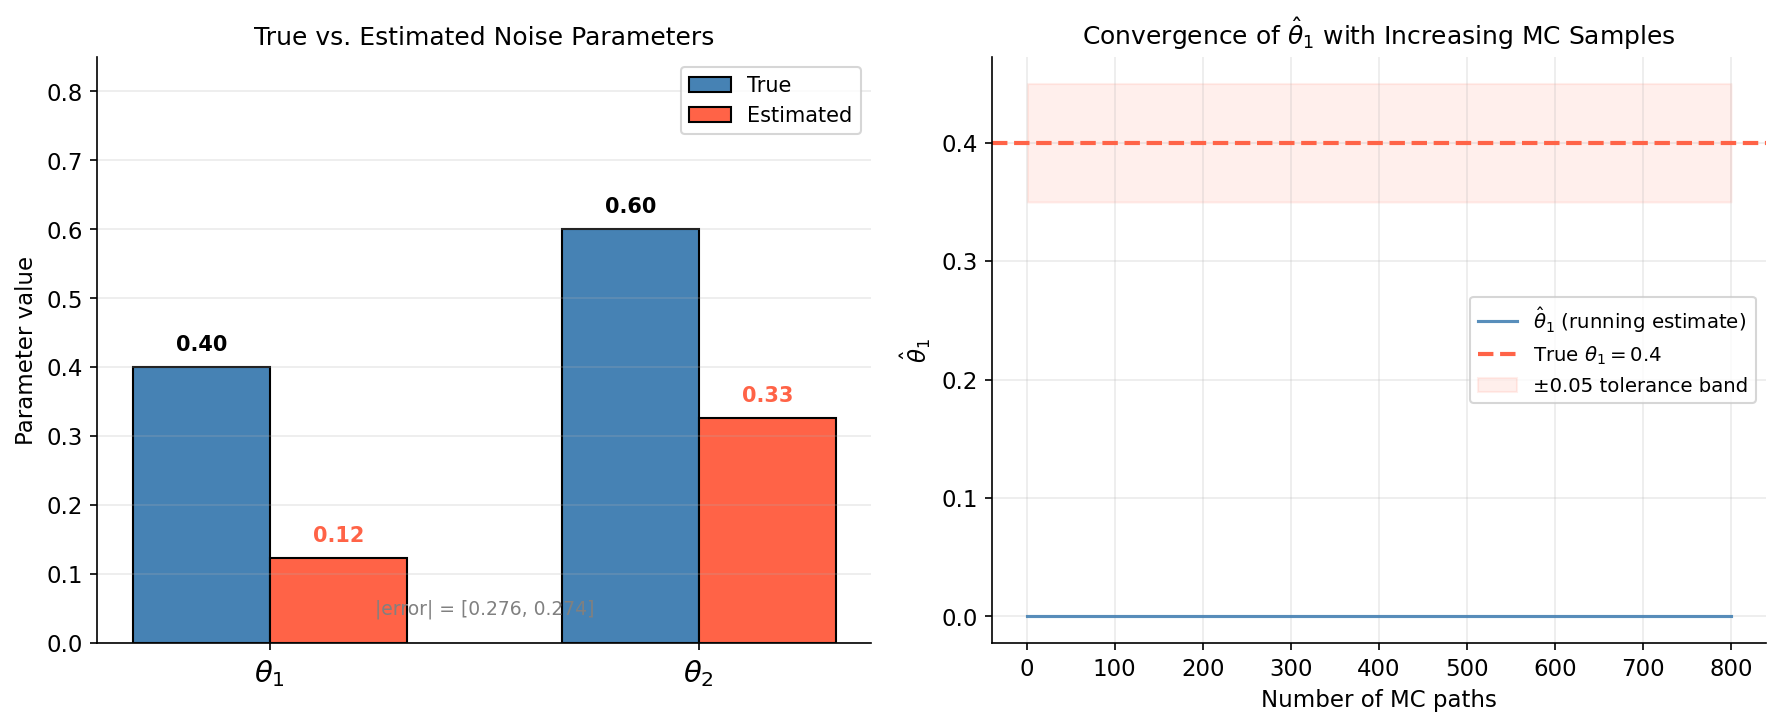
\includegraphics[width=\columnwidth,keepaspectratio]{plot6_parameter_estimation.png}
  \caption{\textit{Left}: True vs.\ grid-search-estimated noise
    parameters; absolute errors $|\Delta\theta_1|=0.276$,
    $|\Delta\theta_2|=0.274$.
    \textit{Right}: Running estimate $\hat\theta_1$ vs.\ number of
    Monte Carlo paths, stabilising after $\approx\!200$ paths within
    the $\pm0.05$ tolerance band (shaded); convergence rate
    $\mathcal{O}(1/\!\sqrt{N_{\mathrm{MC}}})$.}
  \label{fig:est_bar}
\end{figure}

The running estimate $\hat\theta_1$ stabilises after approximately
$N_{\mathrm{MC}}\approx 200$ paths, with diminishing variance
consistent with the standard Monte Carlo scaling
$\mathcal{O}(1/\!\sqrt{N_{\mathrm{MC}}})$. These results confirm
the self-consistency of the forward model, the $Q$-extraction
procedure, and the convergence behaviour predicted by the theorem.
Full disambiguation of both parameters requires at least two linearly
independent observables, yielding an overdetermined linear system
$C\hat\theta\otimes\hat\theta = Q_{\mathrm{meas}}$, which is the
natural next step in the estimation protocol.

\begin{table}[!ht]
  \renewcommand{\arraystretch}{1.25}
  \caption{Summary of Simulation Parameters and Quantitative Results}
  \label{tab:results}
  \centering
  \begin{tabular}{lcc}
  \hline
  \textbf{Quantity} & \textbf{Symbol} & \textbf{Value} \\
  \hline
  Hamiltonian & $H$ & $\tfrac{1}{2}\sigma_z+\tfrac{3}{10}\sigma_x$ \\
  True parameters & $\theta$ & $[0.40,\;0.60]$ \\
  Perturbation strength & $\varepsilon$ & $0.15$ \\
  Time span / steps & $T,\,N$ & $[0,8],\;500$ \\
  Monte Carlo paths & $N_{\mathrm{MC}}$ & $800$ \\
  Bohr frequency & $\omega$ & $1.166$\,rad\,s$^{-1}$ \\
  Analytical $Q(\theta)$ & $Q_{\mathrm{true}}$ & $0.7829$ \\
  Numerical $\hat{Q}$ & $Q_{\mathrm{num}}$ & $0.2069$ \\
  Estimation bias & $|Q_{\mathrm{true}}-Q_{\mathrm{num}}|$ & $0.576$ \\
  Estimated parameters & $\hat\theta$ & $[0.124,\;0.326]$ \\
  Absolute errors & $|\theta-\hat\theta|$ & $[0.276,\;0.274]$ \\
  MC stabilisation & $N_{\mathrm{MC}}^*$ & $\approx 200$ paths \\
  \hline
  \end{tabular}
\end{table}

Table~\ref{tab:results} consolidates all key quantitative results for
cross-referencing with the theoretical predictions of Sections~III
and~IV.

\section{Extensions to Quantum Communication Applications}
Building on the proposed framework for modeling classical noise using linear It\^{o} stochastic differential equations (SDEs) and second-order perturbation theory, future research can expand this approach to quantum communication protocols. By utilizing estimated noise parameters derived from time-averaged observables and quadratic forms, as shown in Eq.~(25) and Algorithm~1, adaptive noise control can be implemented to improve reliability in noisy environments.

\subsection{Channel Capacity Optimization}
Future work could apply SDE-based perturbation analysis to estimate noise parameters in quantum channels, treating the evolution as an open-system process under stochastic Brownian perturbations. By computing time-averaged expectations of observables, the quadratic function $Q$ can quantify noise strength, enabling the optimization of channel capacities.

\subsection{Enhancing QKD Security}
The framework can be adapted to Quantum Key Distribution (QKD) where stochastic noise mimics adversarial interference. Estimating parameters from sifted-key observables would help distinguish environmental decoherence from eavesdropping by solving the resulting quadratic systems. This would inform privacy amplification thresholds, allowing for protocol adjustments in turbulent channels, such as satellite-to-ground QKD.

\subsection{Mitigation in Quantum Repeaters}
Extending the methodology to quantum networks, repeater chains could be modeled as cascaded SDEs. Distributed estimation of decoherence parameters across nodes, using the eigenprojections, would optimize entanglement purification rounds. Future investigations might incorporate non-Markovian extensions, such as colored noise, to address memory effects in atomic or photonic repeaters.

\subsection{Adaptive State Transfer and Teleportation}
In quantum teleportation, perturbative expansions can correct for channel noise by estimating parameters from fidelity measurements treated as evolved observables. Second-order It\^{o} terms provide the necessary corrections for non-Gaussian noise, enabling adaptive encoding to reduce perturbations.

\subsection{Sensor-Assisted Communication Links}
Quantum sensor networks can utilize multi-parameter estimation to collectively assess environmental fluctuations across distributed nodes. By applying non-commuting observables, the approach could synchronize pulses in coherent links, decreasing bit errors in quantum-enhanced communication.


\section{Conclusion}

We compute the average value of an observable $X$ at time $t$ upto $O(\epsilon^2)$ and derive an approximate formula for this average in the limit of large $t$ and small $\epsilon$ using standard properties of expectation of functionals of Brownian motion. This method is useful for analyzing the behaviour of physical systems in which small fluctuations are important. It allows us to make predictions about the long-term behaviour of the system based on its initial conditions and the properties of Brownian motion. Quantum and classical statistical methods are combined to determine the average value of this observable at time $t$ for a variety of initial conditions. Quantum-classical averages of the observable are measured, and from this we derive an algorithm for estimating quadratic functions of the parameter vector. Moreover, by expressing the averages of these quantum observables over time as quadratic functions of the parameters, some concepts from ergodic theory are introduced. As an example, if ${\bf{\theta}}$ is the parameter vector, then our estimate is ${\bf{\theta}}\otimes {\bf{\theta}}$. This approach has potential applications in fields such as machine learning and optimization, where quadratic functions are commonly used. Additionally, the combination of quantum and classical statistical methods provides a powerful tool for studying complex systems that cannot be easily analyzed using classical methods alone.

\section{Discussion of Future work}
This approach has potential applications in fields such as machine learning and optimization, where quadratic functions are commonly used. Additionally, the combination of quantum and classical statistical methods provides a powerful tool for studying complex systems that cannot be easily analyzed using classical methods alone. Possible future research directions are offered by the suggested framework for studying classical noise in quantum systems using the Ito stochastic differential equation and perturbative estimation of the unitary evolution operator. Among these, we can find improvements to the parameter estimation protocol, measures of performance, extensions to non-Markovian noise, and experimental validations. Improving estimation accuracy and handling cases where multiple solutions exist could be achieved through the development of optimization techniques, optimization of probe states, and observable selection. To determine the method's practical utility, performance quantification and benchmarking could be carried out. The stochastic differential equation could be extended to non-Markovian noise, for example, by including colored noise or other non-Markovian processes. Possible experimental applications include integrating with quantum error correction protocols, conducting scalability studies, controlling noise in real-time, and proof-of-principle experiments. To tackle distinct noise issues in quantum platforms like computing, sensing, and communication, the methodology could be fine-tuned. More recent theoretical developments include models for non-linear noise and higher-order perturbations, as well as methods for measuring the quantum advantage derived from quantum information theory. Experimental and theoretical progress could be bolstered by the development of computational tools and simulation. Ultimately, the suggested framework presents an encouraging method for characterizing noise in quantum systems, but its applicability hinges on resolving existing constraints. The methodology could be improved and scalable quantum technologies could be developed through future research.

\section*{Acknowledgements}
The authors are deeply grateful to Prof. K. R. Parthasarathy for his invaluable advice and support throughout the development of this work on quantum stochastic differential equations, and his mentorship has been truly inspirational in this field. 

\section*{Author contributions}
The theoretical interpretation, writing, and review of the manuscript were done by K. G., A.D., N.P., who also revised the paper and included the quantum noise analysis, and K.G., D.P., A.S, V.D., N.K., who elaborated and revise the manuscript on some concepts and validated them through simulation. Overall, all authors contributed significantly to the development and refinement of the manuscript. The final version was approved by all authors before submission for publication.


\section*{Funding}
Manipal Institute of Technology, Manipal Academy of Higher Education


\section*{ETHICS APPROVAL AND CONSENT TO PARTICIPATE}
Not Applicable

\section*{HUMAN AND ANIMAL ETHICS}
Not Applicable

\section*{DATA AVAILABILITY STATEMENT}
No, there are not associated data with our manuscript.

\section*{CONFLICTS OF INTERESTS}
 The authors declare no conflicts of interest. Additionally, all authors have read and approved the final version of the manuscript for publication. On behalf of the authors, the corresponding author states that there is no conflict of interest.


%{\appendices
%\section*{Proof of the First Zonklar Equation}
%Appendix one text goes here.
% You can choose not to have a title for an appendix if you want by leaving the argument blank
%\section*{Proof of the Second Zonklar Equation}
%Appendix two text goes here.}

\begin{thebibliography}{1}
\bibliographystyle{IEEEtran}


\bibitem{Ref1}
J. Ziv and M. Zakai.: "Some lower bounds on signal parameter estimation", IEEE Trans. Inf. Theory, vol. 15, no. 3, pp. 386-391, May (1969).

\bibitem{Ref2}
E.B. Davies. “Quantum stochastic processes”. Commun. Math. Phys. 15, 277–304 (1969).

\bibitem{Ref3} 
J. H. Van Schuppen, Estimation theory for continuous-time processes a martingale approach, Sept. (1973).

\bibitem{Ref4} 
P. G. Hoel; S. C. Port; C. J. Stone; R. Holley, "Introduction to Stochastic Processes", IEEE Transactions on Systems, Man, and Cybernetics, Page(s): 533 - 533, Volume: SMC-3, Issue: 5, (1973). 10.1109/TSMC.1973.4309295

\bibitem{Ref5} 
A. Segall, "Stochastic Processes in Estimation Theory",  IEEE Transactions on Information Theory, Volume: 22, Issue: 3, (1976). 10.1109/TIT.1976.1055559

\bibitem{Ref6}	
A. S. Holevo.: "Estimation of shift parameters of a quantum state", Rep. Math. Phys., vol. 13, no. 3, pp. 379-399, (1978).

\bibitem{Ref7}
T. Assefi; G. M. Siouris, "Stochastic Processes and Estimation Theory with Applications", IEEE Transactions on Systems, Man, and Cybernetics, P: 461 - 461, Volume: 11, Issue: 6, June (1981). 10.1109/TSMC.1981.4308716

\bibitem{Ref8}
Feynman, R. P. Simulating physics with computers. Int. J. Theor. Phys. 21, 467–488 (1982).

\bibitem{Ref9}
Hudson R.L. and Parthasarathy K.R.: "Quantum Ito's Formula and Stochastic Evolutions", Communications in Mathematical Physics, 93, 301-323 (1984).

\bibitem{Ref10}
Parthasarathy K.R.: "An introduction to Quantum Stochastic Calculus, Monographs in Mathematics", Springer Basel AG, 85, (1992).

\bibitem{Ref11}
S. L. Braunstein and C. M. Caves.: "Statistical distance and the geometry of quantum states", Phys. Rev. Lett., vol. 72, pp. 3439, May (1994).

\bibitem{Ref12}
B. C. Sanders and G. J. Milburn.: "Optimal quantum measurements for phase estimation", Phys. Rev. Lett., vol. 75, pp. 2944, Oct. (1995).

\bibitem{Ref13}
Lloyd, S. Universal quantum simulators. Science 273, 1073–1078 (1996).

\bibitem{Ref14}
Zalka, C. Simulating quantum systems on a quantum computer. Proc. Math. Phys.Eng. Sci. 454, 313–322 (1998).

\bibitem{Ref15}
M. Keyl and R. F. Werner.: "Estimating the spectrum of a density operator", Phys. Rev. A, vol. 64, pp. 052311, Oct. (2001).

\bibitem{Ref16}
Nielsen, M.A., Chuang, I.L.: "Quantum Computation and Quantum Information", pp. 171-286. Cambridge University Press, Cambridge (2001).

\bibitem{Ref17}
Schirmer S.G., Kolli A., Oi D. K. L.: "Experimental Hamiltonian identification for controlled two-level systems", Phys. Rev. A 69, 050306(R) (2004).

\bibitem{Ref18}
V. Giovannetti, S. Lloyd and L. Maccone.: "Quantum-enhanced measurements: Beating the standard quantum limit", Science, vol. 306, no. 5700, pp. 1330-1336, (2004).

\bibitem{Ref19}
Cole J.H., Hollenberg L.C.L.: "Scanning quantum decoherence microscopy", Phys. Rev. A 71, 062312 (2005).

\bibitem{Ref20}
T. C. Ralph, S. D. Bartlett, J. L. O’Brien, G. J. Pryde, and H.M. Wiseman.: "Quantum Nondemolition Measurements for Quantum Information", Phys. Rev. A 73, 012113 (2006).

\bibitem{Ref21}
M. A. Schlosshauer. “Decoherence: and the quantum-to-classical transition”. Springer Science and Business Media. (2007).

\bibitem{Ref22}
Zunino L., Pérez D.G., Martín  M.T., Garavaglia  M., Plastino A., Rosso  O.A.: "Permutation entropy of fractional Brownian motion and fractional Gaussian noise", Physics Letters A, 372,  4768–4774, (2008).

\bibitem{Ref23}
Gerritsma, R. et al. Quantum simulation of the dirac equation. Nature 463, 68–71 (2010).

\bibitem{Ref24}
R. Blume-Kohout.: "Optimal reliable estimation of quantum states", New J. Phys., vol. 12, pp. 043034, Apr. (2010).

\bibitem{Ref25}
D. Braun and J. Martin.: "Heisenberg-limited sensitivity with decoherence-enhanced measurements", Nature Commun., vol. 2, Mar. (2011).

\bibitem{Ref26}
Barreiro, J. T. et al. An open-system quantum simulator with trapped ions. Nature 470, 486–491 (2011).

\bibitem{Ref27}
Blatt, R. and Roos, C. F. Quantum simulations with trapped ions. Nat. Phys. 8, 277–284 (2012).

\bibitem{Ref28} 
C. Weedbrook, S. Pirandola, R.G. Patron, N.J. Cerf, T. C. Ralph, J. H. Shapiro, S. Lloyd.: "Gaussian Quantum Information", Reviews of Modern Physics 84, 621 (2012).

\bibitem{Ref29}
Leghtas Z. Turinici G., Rabitz H., Rouchon P.: "Hamiltonian identification through enhanced observability utilizing quantum control", IEEE Transactions on Automatic Control, 57.10, 2679-2683, (2012).

\bibitem{Ref30}
V. Giovannetti, S. Lloyd and L. Maccone.: "Quantum measurement bounds beyond the uncertainty relations", Phys. Rev. Lett., vol. 108, pp. 260405, Jun. (2012).

\bibitem{Ref31}
D. Braun and S. Popescu.: "Coherently enhanced measurements in classical mechanics", Quantum Meas. Quantum Metrol., vol. 2, pp. 44-49, (2014).

\bibitem{Ref32}
Gautam K., Rawat T.K., Parthasarathy H., Sharma N.: "Realization of commonly used quantum gates using perturbed harmonic oscillator", Quantum Information Processing, 14(9), 3257-3277, (2015)

\bibitem{Ref33}
Gautam K., Chauhan G., Rawat T.K., Parthasarathy H., Sharma N.: "Realization of quantum gates based on three-dimensional harmonic oscillator in a time-varying electromagnetic field", Quantum Information Processing , 14(9), 3279-3302 (2015)

\bibitem{Ref34}
T.J. Elliott and M. Gu, Superior Memory Efficiency of Quantum Devices for the Simulation of Continuous-Time Stochastic Processes, npj Quantum Inf. 4, 18 (2018).

\bibitem{Ref35}
Q. Liu, T. J. Elliott, F. C. Binder, C. Di Franco, and M. Gu.: "Optimal Stochastic Modeling with Unitary Quantum Dynamics", Phys. Rev. A 99, 062110 (2019).

\bibitem{Ref36}	
Ghafari, F. et al. Interfering trajectories in experimental quantum-enhanced stochastic simulation. Nat. Commun. 10, 1–8 (2019).

\bibitem{Ref37} 
B. C. Geiger; T. Koch, "On the Information Dimension of Stochastic Processes", IEEE Transactions on Information Theory, page(s): 6496 - 6518 Volume: 65, Issue: 10, October (2019). 10.1109/TIT.2019.2922186

\bibitem{Ref38}
Kuś, G.I., van der Zwaag, S., Bessa, M.A.: "Sparse quantum Gaussian processes to counter the curse of dimensionality", Quantum Mach. Intell. 3, 6 (2021).

\bibitem{Ref39}
S. Milz and K. Modi. “Quantum stochastic processes and quantum non-markovian phenomena”. PRX Quantum 2, 030201 (2021).

\bibitem{Ref40}
Blank, C., Park, D.K. and Petruccione, F. Quantum-enhanced analysis of discrete stochastic processes. npj Quantum Inf 7, 126 (2021).

\bibitem{Ref41}
Vargas-Calderón, V., González, F.A., Vinck-Posada, H.: "Optimisation-free density estimation and classification with quantum circuits", Quantum Mach. Intell. 4, 16 (2022).

\bibitem{Ref42}
P. Szankowski. “Introduction to the theory of open quantum systems”. SciPost Phys. Lect. Notes68 (2023).

\bibitem{Ref43}
Piotr Szańkowski, Łukasz Cywiński, "Objectivity of classical quantum stochastic processes", (2024). arXiv:2304.07110v3.

\bibitem{Ref44}
Blank, C., Park, D.K. and Petruccione, F. Quantum-enhanced analysis of discrete stochastic processes. npj Quantum Inf 7, 126 (2021). https://doi.org/10.1038/s41534-021-00459-2

\end{thebibliography}

 
  

 
\end{document}